\begin{figure}[!htbp]
\centering
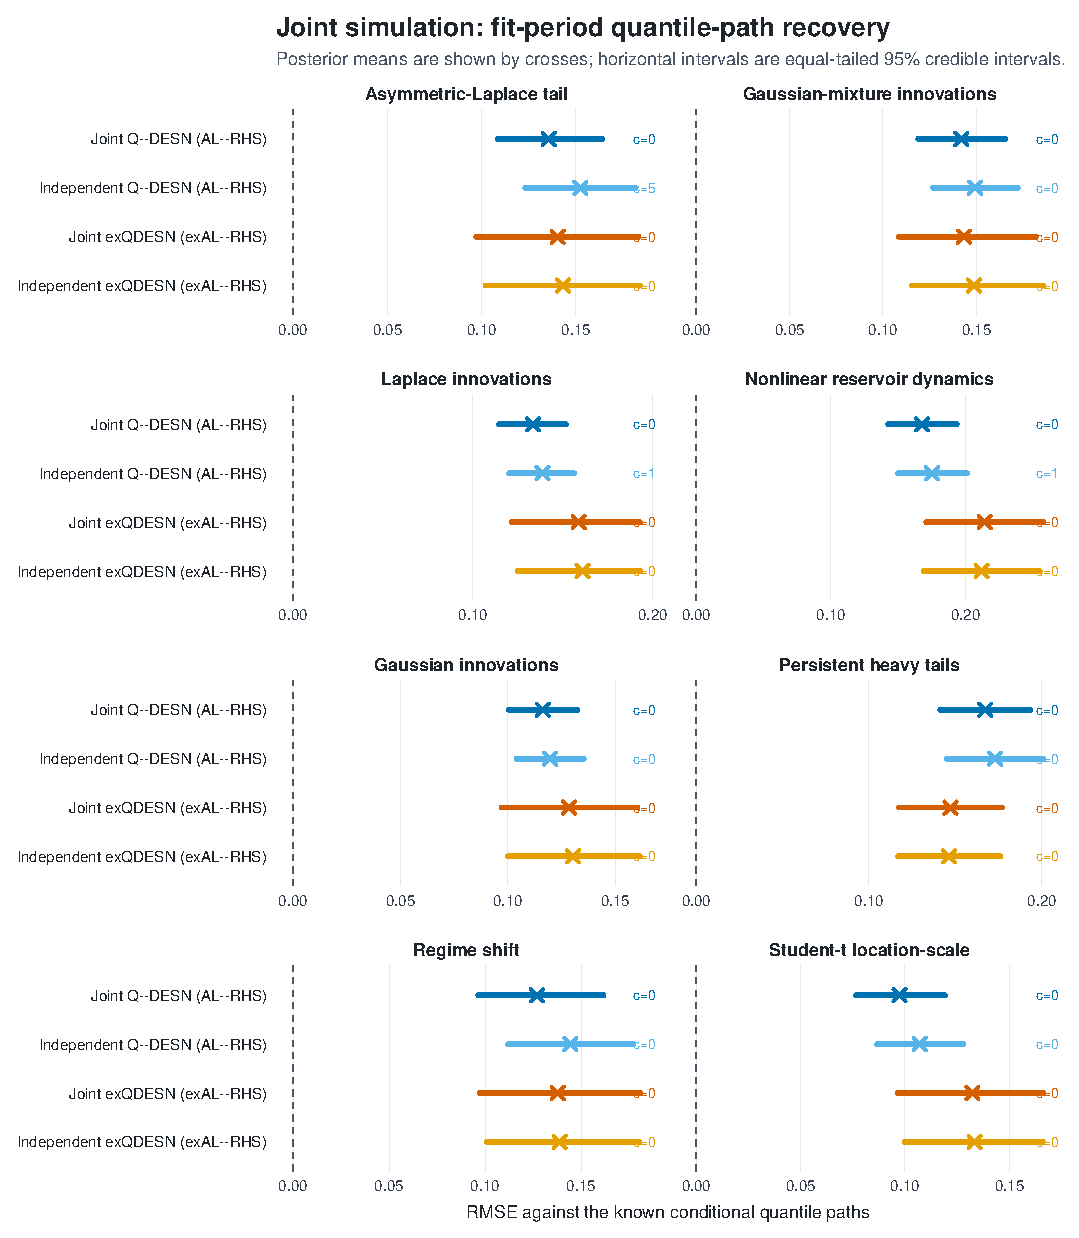
\includegraphics[width=0.94\textwidth]{figures/joint_qdesn_simulation/joint_qdesn_phase181_fit_oracle_rmse_intervals.pdf}
\caption{Posterior fitting-sample recovery of the known conditional quantile
paths in the joint simulation. Crosses show posterior means and horizontal bars
show equal-tailed 95\% credible intervals from 8,000 retained MCMC draws per
comparison after monotone rearrangement; lower is better. Right-hand labels
give raw crossing counts in the posterior-mean fitted grid before
rearrangement; all counts after rearrangement are zero.}
\label{fig:joint-qdesn-phase181-fit-rmse-intervals}
\end{figure}
